%===============================================================================
% LaTeX sjabloon voor de bachelorproef toegepaste informatica aan HOGENT
% Meer info op https://github.com/HoGentTIN/latex-hogent-report
%===============================================================================

\documentclass[dutch,dit,thesis]{hogentreport}

% TODO:
% - If necessary, replace the option `dit`' with your own department!
%   Valid entries are dbo, dbt, dgz, dit, dlo, dog, dsa, soa
% - If you write your thesis in English (remark: only possible after getting
%   explicit approval!), remove the option "dutch," or replace with "english".

\usepackage{lipsum} % For blind text, can be removed after adding actual content

%% Pictures to include in the text can be put in the graphics/ folder
\graphicspath{{graphics/}}

%% For source code highlighting, requires pygments to be installed
%% Compile with the -shell-escape flag!
\usepackage[section]{minted}
%% If you compile with the make_thesis.{bat,sh} script, use the following
%% import instead:
%% \usepackage[section,outputdir=../output]{minted}
\usemintedstyle{solarized-light}
\definecolor{bg}{RGB}{253,246,227} %% Set the background color of the codeframe

%% Change this line to edit the line numbering style:
\renewcommand{\theFancyVerbLine}{\ttfamily\scriptsize\arabic{FancyVerbLine}}

%% Macro definition to load external java source files with \javacode{filename}:
\newmintedfile[javacode]{java}{
    bgcolor=bg,
    fontfamily=tt,
    linenos=true,
    numberblanklines=true,
    numbersep=5pt,
    gobble=0,
    framesep=2mm,
    funcnamehighlighting=true,
    tabsize=4,
    obeytabs=false,
    breaklines=true,
    mathescape=false
    samepage=false,
    showspaces=false,
    showtabs =false,
    texcl=false,
}

% Other packages not already included can be imported here

%%---------- Document metadata -------------------------------------------------
% TODO: Replace this with your own information
\author{Ernst Aarden}
\supervisor{Dhr. F. Van Houte}
\cosupervisor{Mevr. S. Beeckman}
\title[Optionele ondertitel]%
    {Titel van de bachelorproef}
\academicyear{\advance\year by -1 \the\year--\advance\year by 1 \the\year}
\examperiod{1}
\degreesought{\IfLanguageName{dutch}{Professionele bachelor in de toegepaste informatica}{Bachelor of applied computer science}}
\partialthesis{false} %% To display 'in partial fulfilment'
%\institution{Internshipcompany BVBA.}

%% Add global exceptions to the hyphenation here
\hyphenation{back-slash}

%% The bibliography (style and settings are  found in hogentthesis.cls)
\addbibresource{bachproef.bib}            %% Bibliography file
\addbibresource{../voorstel/voorstel.bib} %% Bibliography research proposal
\defbibheading{bibempty}{}

%% Prevent empty pages for right-handed chapter starts in twoside mode
\renewcommand{\cleardoublepage}{\clearpage}

\renewcommand{\arraystretch}{1.2}

%% Content starts here.
\begin{document}

%---------- Front matter -------------------------------------------------------

\frontmatter

\hypersetup{pageanchor=false} %% Disable page numbering references
%% Render a Dutch outer title page if the main language is English
\IfLanguageName{english}{%
    %% If necessary, information can be changed here
    \degreesought{Professionele Bachelor toegepaste informatica}%
    \begin{otherlanguage}{dutch}%
       \maketitle%
    \end{otherlanguage}%
}{}

%% Generates title page content
\maketitle
\hypersetup{pageanchor=true}

%%=============================================================================
%% Voorwoord
%%=============================================================================

\chapter*{\IfLanguageName{dutch}{Woord vooraf}{Preface}}%
\label{ch:voorwoord}

%% TODO:
%% Het voorwoord is het enige deel van de bachelorproef waar je vanuit je
%% eigen standpunt (``ik-vorm'') mag schrijven. Je kan hier bv. motiveren
%% waarom jij het onderwerp wil bespreken.
%% Vergeet ook niet te bedanken wie je geholpen/gesteund/... heeft

\lipsum[1-2]
%%=============================================================================
%% Samenvatting
%%=============================================================================

% TODO: De "abstract" of samenvatting is een kernachtige (~ 1 blz. voor een
% thesis) synthese van het document.
%
% Een goede abstract biedt een kernachtig antwoord op volgende vragen:
%
% 1. Waarover gaat de bachelorproef?
% 2. Waarom heb je er over geschreven?
% 3. Hoe heb je het onderzoek uitgevoerd?
% 4. Wat waren de resultaten? Wat blijkt uit je onderzoek?
% 5. Wat betekenen je resultaten? Wat is de relevantie voor het werkveld?
%
% Daarom bestaat een abstract uit volgende componenten:
%
% - inleiding + kaderen thema
% - probleemstelling
% - (centrale) onderzoeksvraag
% - onderzoeksdoelstelling
% - methodologie
% - resultaten (beperk tot de belangrijkste, relevant voor de onderzoeksvraag)
% - conclusies, aanbevelingen, beperkingen
%
% LET OP! Een samenvatting is GEEN voorwoord!

%%---------- Nederlandse samenvatting -----------------------------------------
%
% TODO: Als je je bachelorproef in het Engels schrijft, moet je eerst een
% Nederlandse samenvatting invoegen. Haal daarvoor onderstaande code uit
% commentaar.
% Wie zijn bachelorproef in het Nederlands schrijft, kan dit negeren, de inhoud
% wordt niet in het document ingevoegd.

\IfLanguageName{english}{%
\selectlanguage{dutch}
\chapter*{Samenvatting}
\lipsum[1-4]
\selectlanguage{english}
}{}

%%---------- Samenvatting -----------------------------------------------------
% De samenvatting in de hoofdtaal van het document

\chapter*{\IfLanguageName{dutch}{Samenvatting}{Abstract}}

\lipsum[1-4]


%---------- Inhoud, lijst figuren, ... -----------------------------------------

\tableofcontents

% In a list of figures, the complete caption will be included. To prevent this,
% ALWAYS add a short description in the caption!
%
%  \caption[short description]{elaborate description}
%
% If you do, only the short description will be used in the list of figures

\listoffigures

% If you included tables and/or source code listings, uncomment the appropriate
% lines.
%\listoftables
%\listoflistings

% Als je een lijst van afkortingen of termen wil toevoegen, dan hoort die
% hier thuis. Gebruik bijvoorbeeld de ``glossaries'' package.
% https://www.overleaf.com/learn/latex/Glossaries

%---------- Kern ---------------------------------------------------------------

\mainmatter{}

% De eerste hoofdstukken van een bachelorproef zijn meestal een inleiding op
% het onderwerp, literatuurstudie en verantwoording methodologie.
% Aarzel niet om een meer beschrijvende titel aan deze hoofdstukken te geven of
% om bijvoorbeeld de inleiding en/of stand van zaken over meerdere hoofdstukken
% te verspreiden!

%%=============================================================================
%% Inleiding
%%=============================================================================

\chapter{\IfLanguageName{dutch}{Inleiding}{Introduction}}%
\label{ch:inleiding}

This bachelor thesis is written based on a business case from TrustBuilder, a European company providing Identity and Access Management (IAM) solutions for organizations across Europe, with extensive customization capabilities to satisfy client-specific needs.

Their product, also named TrustBuilder, is a platform that aims to be able to handle any IAM need, such as authentication, session management, authorization, and user management. Further requirements can take many forms, and the TrustBuilder platform needs to be able to tightly integrate with each client’s user-facing applications and other services. As these needs may differ from application to application, not everything can be a native part of the IAM system, and customization capabilities are a must. To satisfy these needs, their clients need to be able to to customize and extend their platform using custom code.

TrustBuilder tackles this problem by allowing for the creation of \emph{workflows}. These workflows consist of simple building blocks such as \emph{script blocks}, \emph{adapters} and \emph{services}, using arrow connectors and \emph{condition blocks} between them for control flow. Script blocks can run custom JavaScript functions, allowing workflows to be used to implement virtually any functionality missing from the base product, as well as interface with the base product directly.

\section{\IfLanguageName{dutch}{Probleemstelling}{Problem Statement}}%
\label{sec:probleemstelling}

TrustBuilder wants to overhaul their workflow platform to improve the developer experience and maintainability of workflows. Therefore, they want to know what language(s) their workflow platform should be built around. Currently, JavaScript is used to script these extensions, but this decision was made over a decade ago and needs to be re-evaluated.

\section{\IfLanguageName{dutch}{Onderzoeksvraag}{Research question}}%
\label{sec:onderzoeksvraag}

This thesis will investigate which languages would be the best choice for scripting extensions and customizations for the TrustBuilder IAM platforms. This encompasses the following sub-questions: 
\begin{itemize}
    \item{What are the key indicators these languages should be evaluated against?}
    \item{What would be the pros and cons of specific language choices?}
    \item{What are the security implications of specific language choices?}
\end{itemize}

\section{\IfLanguageName{dutch}{Onderzoeksdoelstelling}{Research objective}}%
\label{sec:onderzoeksdoelstelling}

A primary language choice based on the performed research and a proof of concept showcasing the language’s suitability for IAM-related tasks will allow TrustBuilder to start the overhaul of workflows with certainty.
This thesis aims to provide insight into the process behind that selection, the advantages and disadvantages of its use, and compare it to a secondary contender. Both the primary and secondary language choices will be put to the test in a proof of concept that covers typical use cases of TrustBuilder's current extension system.

\section{\IfLanguageName{dutch}{Opzet van deze bachelorproef}{Structure of this bachelor thesis}}%
\label{sec:opzet-bachelorproef}

The remainder of this bachelor thesis is structured as follows:

In chapter~\ref{ch:stand-van-zaken}, an overview of the state of the art of the research domain is given, based on a literature review.

In chapter~\ref{ch:methodologie}, the methodology is explained, and the research methods used to formulate an answer to the research question are discussed.

In chapter~\ref{ch:requirements}, the requirements of the final language choice are discussed. A long list of options is evaluated against these requirements to create a short list of two languages which will each be used in a proof of concept.

In chapter~\ref{ch:proof-of-concept}, each of the two languages in the short list are used to create a proof of concept which covers common use cases for TrustBuilder's extension system, and the findings in making these will be discussed.

Finally, in chapter ~\ref{ch:conclusie}, a conclusion and an answer to the research question is given, with a primary and secondary language choice and a summary of the reasons behind it.

\chapter{\IfLanguageName{dutch}{Stand van zaken}{State of the art}}%
\label{ch:stand-van-zaken}

% Tip: Begin elk hoofdstuk met een paragraaf inleiding die beschrijft hoe
% dit hoofdstuk past binnen het geheel van de bachelorproef. Geef in het
% bijzonder aan wat de link is met het vorige en volgende hoofdstuk.

% Pas na deze inleidende paragraaf komt de eerste sectiehoofding.

To gain a deeper understanding of the research problem and the context in which it exists, this chapter explores the technologies involved, the current state of programming language popularity, and the approaches taken by comparable services.

\section{IAM standards}
To attain further insight in the problem space, it is important to briefly discuss the dominant IAM standards. According to \textcite{Naik2016}, the most established identity protocols in the cloud computing industry are the following three: Security Assertion Markup Language (SAML), OAuth, and OpenID Connect (OIDC). 

\subsection{SAML}
Security Assertion Markup Language (SAML) and its associated protocols form an open standard for communicating information, ``packaged'' in an \emph{assertion}, about a subject, such as a user \autocite{Kemp2005}. SAML assertions, provided by an \emph{identity provider} (IdP), may represent authentication information, authorization decisions, or attributes associated with the subject. A \emph{service provider} (SP) can then use these assertions for access control and identification.

The use of SAML 2.0 can support single sign-on (SSO) for browsers, as specified by the Web Browser SSO Profile \autocite{Hughes2005}. When an unauthenticated HTTP user agent, in this case a browser, requests a secured resource from a service provider, the SP issues a SAML authentication request to be delivered to the identity provider by the user agent. The IdP identifies the subject, and issues a SAML response to be delivered back to the service provider by the user agent. The service provider can then establish a security context for the subject and return the requested resource. 

\subsection{OAuth}
``The OAuth 2.0 authorization framework enables a third-party
application to obtain limited access to an HTTP service, either on
behalf of a resource owner [...], or [...] on its own behalf'' \autocite{Hardt2023}.

A typical OAuth flow consists of a \emph{client} (e.g. an application) requesting authorization from a \emph{resource owner}. When the resource owner issues an \emph{authorization grant} to the client, it may then exchange that authorization grant for an \emph{access token} from an authorization server. Using that access token, it may then access a protected resource, owned by the resource owner, on the resource server. \autocite{Hardt2023}
\begin{figure}[h]
    \begin{scriptsize}
        \begin{verbatim} 
            +--------+                               +---------------+
            |        |--(A)- Authorization Request ->|   Resource    |
            |        |                               |     Owner     |
            |        |<-(B)-- Authorization Grant ---|               |
            |        |                               +---------------+
            |        |
            |        |                               +---------------+
            |        |--(C)-- Authorization Grant -->| Authorization |
            | Client |                               |     Server    |
            |        |<-(D)----- Access Token -------|               |
            |        |                               +---------------+
            |        |
            |        |                               +---------------+
            |        |--(E)----- Access Token ------>|    Resource   |
            |        |                               |     Server    |
            |        |<-(F)--- Protected Resource ---|               |
            +--------+                               +---------------+
        \end{verbatim}
    \end{scriptsize}
    \caption{Abstract Protocol Flow \autocite{Hardt2023}}
\end{figure}

JSON Web Tokens (JWTs) may be used both as OAuth 2.0 authentication grants and tokens \autocite{Jones2015a, Bertocci2021}. They provide a secure way to communicate information (referred to as claims) about a subject, encoded as a JSON object which may be signed and/or encrypted. \autocite{Jones2015}

\subsection{OpenID Connect}
As detailed by its specification, OpenID Connect (OIDC) is ``a simple identity layer on top of the OAuth 2.0 protocol''. Information about the end user is conveyed in claims, as part of a JWT called the ID token. This information can then be used by a client to authenticate the user. \autocite{Sakimura2014} 

\section{Server-side languages}
\subsection{Language characteristics}
Before discussing individual programming languages
\subsubsection{Memory Safety}
% TODO: Explain memory safety and security impact

\subsubsection{Type systems}
% TODO: Explain static and dynamic typing, impact on bugs

\subsection{Popular server-side programming languages}
To determine possibly suitable programming languages, surveys may provide useful data to determine the currently most popular ones. The Stack Overflow Developer Survey 2023 \autocite{StackOverflow2023} and The State of Developer Ecosystem 2023 \autocite{JetBrains2023} each provide statistics on programming language popularity. Based on these results, the four most popular server-side programming languages are JavaScript, Python, Java, and TypeScript. Further popular languages include C, C++, C\#, PHP, Go, Kotlin, and Rust.

\subsubsection{JavaScript and TypeScript}
In both surveys, JavaScript proves to be the most widely used programming language across developers. Despite having originally been created for usage in browsers \autocite{NCC1995}, it can also be used in server-side environments on runtime systems such as Node.js \autocite{OpenJSFoundation}.

According to the TypeScript Handbook, TypeScript is a typed superset of JavaScript \autocite{TypeScript2023}. Its compiler checks code for type errors, and will then produce plain JavaScript code. This allows the compiled code to be run in any JS runtime environment.

\subsubsection{Python}
Python is a general-purpose programming language designed with simplicity and readability in mind \autocite{Peters2004}. Based on GitHub's 2022 Octoverse report, \textcite{Scarlett2023} states that Python is commonly used for web and software development, task automation, machine learning and data science, financial analysis, and artificial intelligence.

The official Python documentation describes it as being ``suitable as an extension language for customizable applications'' \autocite{PSF2023}.

\subsubsection{Java}
Java is a general-purpose object-oriented programming language \autocite{Lindholm2015}. A Java application may be compiled to instructions for the Java Virtual Machine (JVM), which allows the language to be hardware- and operating system-independent. Other popular JVM languages include Kotlin and Scala \autocite{StackOverflow2023, JetBrains2023}.

\subsubsection{WebAssembly}
As stated on its home page, ``WebAssembly (abbreviated Wasm) is a binary instruction format [...] designed as a portable compilation target for programming languages, enabling deployment on the web for client and server applications'' \autocite{WebAssembly}. Although it is not a programming language itself, a runtime environment that can run Wasm applications would be able to run applications written in a variety of languages, such as C, C++, and Rust \autocite{EmscriptenContributors2015, RWWG2023}.

\section{Current approach}
TrustBuilder's current technology for allowing customization and extension of their platform are called workflows \autocite{DefiningWorkflows}. Workflows consist of elements, such as conditions, scripts, and adapters, which are executed in an order defined by their connections. Custom code can be written in the form of JavaScript functions, which can be executed by script elements. Java code can also be uploaded as a ``service'' JAR file to the workflow platform, which can then be called from within a JavaScript function.

\section{Comparable services}
\subsection{Auth0 Actions}
Auth0 is an IAM platform that enables developers to add authentication and authorization services to their applications \autocite{Auth0Overview}. Actions, one of their customization capabilities, let customers ``customize and extend Auth0's capabilities with custom logic'' \autocite{Auth0Actions}. Auth0 Actions are independent Node.js JavaScript functions which can be executed at specific points in identity flows. These functions typically take two parameters as input: an event object, describing an interaction with the platform, and an API object, providing the function implementation with the ability to determine the outcome of the flow, or call other Auth0 APIs relevant to the flow \autocite{Auth0Triggers}. These function are also able to use dependencies from the npm package registry.



\subsection{Cloudflare Workers}
A more general-purpose example, Cloudflare Workers, announced by Kenton \textcite{Varda2017}, were created to allow customers to run code on Cloudflare's edge network, to cover use cases Cloudflare themselves can't. A Cloudflare Worker could initially only be written in JavaScript, but can now run code written in any language that compiles to JavaScript (such as TypeScript, Python, and Kotlin) or WebAssembly (such as C, C++, Rust and Go). \autocite{Varda2018, Koeninger2020}

\subsection{GitHub Actions}
GitHub Actions, GitHub's CI/CD platform, allows for the execution of logic when certain events take place within a GitHub repository \autocite{GitHubActions}. Although this is aimed more at DevOps workflows, it serves as another example of platforms providing extensibility and customizability for their clients. An Actions workflow consists of ``jobs'', which contain a series of steps. These steps can either be shell scripts or actions. Actions are reusable units of logic, and can be created by any user \autocite{GitHubCustomActions}. There are three types of actions:
\begin{itemize}
    \item{JavaScript actions} 
    \item{Docker container actions, allowing more freedom in terms of operating systems, tools and language choice.}
    \item{Composite Actions, consisting of multiple workflow steps}
\end{itemize}
Actions take input parameters as environment variables, and provide outputs by setting environment variables. 

%%=============================================================================
%% Methodologie
%%=============================================================================

\chapter{\IfLanguageName{dutch}{Methodologie}{Methodology}}%
\label{ch:methodologie}

%% TODO: In dit hoofstuk geef je een korte toelichting over hoe je te werk bent
%% gegaan. Verdeel je onderzoek in grote fasen, en licht in elke fase toe wat
%% de doelstelling was, welke deliverables daar uit gekomen zijn, en welke
%% onderzoeksmethoden je daarbij toegepast hebt. Verantwoord waarom je
%% op deze manier te werk gegaan bent.
%% 
%% Voorbeelden van zulke fasen zijn: literatuurstudie, opstellen van een
%% requirements-analyse, opstellen long-list (bij vergelijkende studie),
%% selectie van geschikte tools (bij vergelijkende studie, "short-list"),
%% opzetten testopstelling/PoC, uitvoeren testen en verzamelen
%% van resultaten, analyse van resultaten, ...
%%
%% !!!!! LET OP !!!!!
%%
%% Het is uitdrukkelijk NIET de bedoeling dat je het grootste deel van de corpus
%% van je bachelorproef in dit hoofstuk verwerkt! Dit hoofdstuk is eerder een
%% kort overzicht van je plan van aanpak.
%%
%% Maak voor elke fase (behalve het literatuuronderzoek) een NIEUW HOOFDSTUK aan
%% en geef het een gepaste titel.

The research will be divided into 6 phases, the first of which is a literature review. Literature research will be performed to examine existing approaches, explore popular languages, and gain a deeper understanding of the state of the art. The result of this literature search can be found in section 2 of this research proposal.

Phase 2 consists of creating a list of minimal requirements for a suitable language choice. Possible types of requirements could include ease of use, security implications, performance, and suitability for IAM-related tasks. A concrete list of measurable requirements will be assembled in consultation with thesis stakeholders and employees at TrustBuilder. The MoSCoW method will be used to order these requirements by importance, and each requirement will be marked as functional or non-functional.

Phase 3 is to create a long list of options, checked against the previously listed requirements. The literature review from phase 1 will be used to build an exhaustive list of suitable language choices. Popular existing options, as well as possibly lesser-known choices, will be considered.

Phase 4 aims to create a short list of the three most promising options, using a requirements summary table.

In phase 5, a proof of concept will be created to validate the suitability of each language in the short list. The proof of concept will consist of a simple HTTP server for each chosen language, which will allow running code that handles HTTP requests in the specified language. Three scripts will be written for each language, and will handle three distinct needs. The exact functionality of these three types of scripts will be decided based on TrustBuilder's typical customization requirements. This proof of concept will help further solidify and compare each language's suitability for customizing and extending IAM systems, and will provide deeper insight in their tooling and ease of use for these purposes.

Phase 6 will consist of drawing conclusions out of the research and propose next steps. The results and findings from the previous phases will be analyzed, and limitations and areas for future research will be identified.

Throughout this entire process, a thesis will be written that documents the research, findings, and proposed solutions.

\begin{figure}[h]
    \centering
    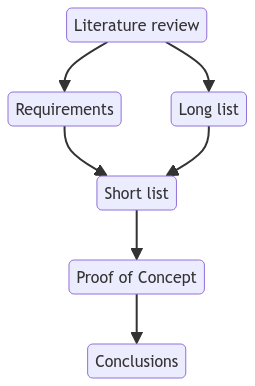
\includegraphics[height=.3\paperheight]{methodology.png}
    \caption{A flowchart representation of the methodology}
\end{figure}


% Voeg hier je eigen hoofdstukken toe die de ``corpus'' van je bachelorproef
% vormen. De structuur en titels hangen af van je eigen onderzoek. Je kan bv.
% elke fase in je onderzoek in een apart hoofdstuk bespreken.

%\input{...}
%\input{...}
%...

%%=============================================================================
%% Conclusie
%%=============================================================================

\chapter{\IfLanguageName{dutch}{Conclusie}{Conclusion}}%
\label{ch:conclusie}

% TODO: Trek een duidelijke conclusie, in de vorm van een antwoord op de
% onderzoeksvra(a)g(en). Wat was jouw bijdrage aan het onderzoeksdomein en
% hoe biedt dit meerwaarde aan het vakgebied/doelgroep? 
% Reflecteer kritisch over het resultaat. In Engelse teksten wordt deze sectie
% ``Discussion'' genoemd. Had je deze uitkomst verwacht? Zijn er zaken die nog
% niet duidelijk zijn?
% Heeft het onderzoek geleid tot nieuwe vragen die uitnodigen tot verder 
%onderzoek?

\lipsum[76-80]



%---------- Bijlagen -----------------------------------------------------------

\appendix

\chapter{Onderzoeksvoorstel}

Het onderwerp van deze bachelorproef is gebaseerd op een onderzoeksvoorstel dat vooraf werd beoordeeld door de promotor. Dat voorstel is opgenomen in deze bijlage.

%% TODO: 
%\section*{Samenvatting}

% Kopieer en plak hier de samenvatting (abstract) van je onderzoeksvoorstel.

% Verwijzing naar het bestand met de inhoud van het onderzoeksvoorstel
%---------- Inleiding ---------------------------------------------------------

\section{Introduction}%
\label{sec:introduction}

This research proposal is written based on a business case of TrustBuilder, a European company providing Identity and Access Management (IAM) solutions for organizations across Europe, with extensive customization capabilities to satisfy client-specific needs.

Their product, also named TrustBuilder, is platform that aims to be able to handle any IAM need, such as authentication, session management, authorization, and user management. Further requirements can take many forms, and the TrustBuilder platform needs to be able to tightly integrate with each client’s user-facing applications and other services. As these needs may differ from application to application, not everything can be a native part of the IAM system, and customization capabilities are a must. In order to satisfy these needs, their clients need to be able to to customize and extend their platform using custom code.

To tackle this problem, TrustBuilder allows for the creation of “workflows”. These workflows consist of simple building blocks such as “script blocks”, “adapters” and “services”, using arrow connectors and “condition” blocks between them for control flow. Script blocks can run custom JavaScript functions, allowing workflows to be used to implement virtually any functionality missing from the base product, as well as integrate with the base product directly.

TrustBuilder wants to overhaul their workflow platform to improve the developer experience and maintainability of workflows. Therefore, they want to know what language(s) their workflow platform should be built around.

This thesis will investigate which languages would be the best choice for scripting extensions and customizations for IAM platforms. A primary language choice based on the performed research and a proof of concept showcasing the language’s suitability for IAM-related tasks will allow TrustBuilder to start the overhaul of workflows with certainty.

%---------- Stand van zaken ---------------------------------------------------

\section{State of the art}%
\label{sec:state-of-the-art}

\subsection{Comparable services}
\subsubsection{Auth0 Actions}
Auth0 is an IAM platform that enables developers to add authentication and authorization services to their applications \autocite{Auth0Overview}. Actions, one of their customization capabilities, let customers ``customize and extend Auth0's capabilities with custom logic'' \autocite{Auth0Actions}. Auth0 Actions are Node.JS JavaScript functions which can be executed at specific points in identity flows.

\subsubsection{Cloudflare Workers}
A more general-purpose example, Cloudflare Workers, announced by Kenton \textcite{Varda2017}, were created to allow their customers to run code on Cloudflare's edge network, to cover use cases Cloudflare themselves can't. A Cloudflare Worker could initially only be written in JavaScript, but can now run code written in any language that compiles to JavaScript (such as TypeScript, Python, and Kotlin) or WebAssembly (such as C, C++, Rust and Go). \autocite{Varda2018, Koeninger2020}

\subsection{Server-side languages}
To determine possibly suitable programming languages, surveys may provide useful data to determine the currently most popular ones. The Stack Overflow Developer Survey 2023 \autocite{StackOverflow2023} and The State of Developer Ecosystem 2023 \autocite{JetBrains2023} each provide statistics on programming language popularity. Based on these results, the four most popular Server-side programming languages are JavaScript, Python, Java, and TypeScript. Further popular languages include   C C++, C\#, PHP, Go, Kotlin, and Rust.

\subsubsection{JavaScript and TypeScript}
In both surveys, JavaScript proves to be the most widely used programming language across developers. Despite having originally been created for usage in browsers \autocite{NCC1995}, it can also be used in server-side environments on runtime systems such as Node.js \autocite{OpenJSFoundation}.

According to the TypeScript Handbook, TypeScript is a typed superset of JavaScript \autocite{TypeScript2023}. Its compiler checks code for type errors, and will then produce plain JavaScript code. This allows the compiled code to be run in any JS runtime environment.

\subsubsection{Python}
Python is a general-purpose programming language designed with simplicity and readability in mind \autocite{Peters2004}. Based on GitHub's 2022 Octoverse report, \textcite{Scarlett2023} states that Python is commonly used for web and software development, task automation, machine learning and data science, financial analysis, and artificial intelligence.

The official Python documentation describes it as being ``suitable as an extension language for customizable applications'' \autocite{PSF2023}.

\subsubsection{Java}
Java is a general-purpose object-oriented programming language \autocite{Lindholm2015}. A Java application may be compiled to instructions for the Java Virtual Machine (JVM), which allows the language to be hardware- and operating system-independent. Other popular JVM languages include Kotlin and Scala \autocite{StackOverflow2023, JetBrains2023}.

\subsubsection{WebAssembly}
As stated on its home page, ``WebAssembly (abbreviated Wasm) is a binary instruction format [...] designed as a portable compilation target for programming languages, enabling deployment on the web for client and server applications'' \autocite{WebAssembly}. Although it is not a programming language itself, a runtime environment that can run Wasm applications would be able to run applications written in a variety of languages.

\subsection{IAM standards}
To gain a deeper understanding of the problem space, it is important to briefly discuss the dominant IAM technologies. According to \textcite{Naik2016}, the most established identity protocols in the cloud computing industry are the following three: Security Assertion Markup Language (SAML), OAuth, and OpenID Connect (OIDC). 

\subsubsection{SAML}
Security Assertion Markup Language (SAML) and its associated protocols form an open standard for communicating information, ``packaged'' in an \emph{assertion}, about a subject, such as a user \autocite{Kemp2005}. SAML assertions, provided by an \emph{identity provider}, may represent authentication information, authorization decisions, or attributes associated with the subject. A \emph{service provider} can then use these assertions for access control and identification.

The use of SAML 2.0 can support single sign-on (SSO) of browsers, as specified by the Web Browser SSO Profile \autocite{Hughes2005}. When an unauthenticated HTTP user agent, in this case a browser, requests a secured resource from a service provider, the service provider issues a SAML authentication request to be delivered to the identity provider by the user agent. The identity provider identifies the subject, and issues a SAML response to be delivered to the service provider by the user agent. The service provider can then establish a security context for the subject and return the requested resource. 

\subsubsection{OAuth}
``The OAuth 2.0 authorization framework enables a third-party
application to obtain limited access to an HTTP service, either on
behalf of a resource owner [...], or [...] on its own behalf.'' \autocite{Hardt2023}


A typical OAuth flow consists of a \emph{client} (e.g. an application) requesting authorization from a \emph{resource owner}. When the resource owner issues an \emph{authorization grant} to the client, it may then exchange that authorization grant for an \emph{access token} from an authorization server. Using that access token, it may then access a protected resource, owned by the resource owner, on the resource server. \autocite{Hardt2023}
\begin{figure}[h]
\begin{scriptsize}
\begin{verbatim} 
+--------+                               +---------------+
|        |--(A)- Authorization Request ->|   Resource    |
|        |                               |     Owner     |
|        |<-(B)-- Authorization Grant ---|               |
|        |                               +---------------+
|        |
|        |                               +---------------+
|        |--(C)-- Authorization Grant -->| Authorization |
| Client |                               |     Server    |
|        |<-(D)----- Access Token -------|               |
|        |                               +---------------+
|        |
|        |                               +---------------+
|        |--(E)----- Access Token ------>|    Resource   |
|        |                               |     Server    |
|        |<-(F)--- Protected Resource ---|               |
+--------+                               +---------------+
\end{verbatim}
\end{scriptsize}
\caption{Abstract Protocol Flow \autocite{Hardt2023}}
\end{figure}

A JSON Web Token (JWT) may be used as both as OAuth 2.0 authentication grants and tokens \autocite{Jones2015a, Bertocci2021}. It provides a secure way to communicate information about a subject (referred to as claims), encoded as a JSON object which may be signed and/or encrypted. \autocite{Jones2015}

\subsubsection{OpenID Connect}
As detailed by its specification, OpenID Connect (OIDC) is ``a simple identity layer on top of the OAuth 2.0 protocol''. Information about the end user is conveyed in claims, as part of a JWT called an ID token. This information can then be used by a client to authenticate the user. \autocite{Sakimura2014} 

% Voor literatuurverwijzingen zijn er twee belangrijke commando's:
% \autocite{KEY} => (Auteur, jaartal) Gebruik dit als de naam van de auteur
%   geen onderdeel is van de zin.
% \textcite{KEY} => Auteur (jaartal)  Gebruik dit als de auteursnaam wel een
%   functie heeft in de zin (bv. ``Uit onderzoek door Doll & Hill (1954) bleek
%   ...'')

%---------- Methodologie ------------------------------------------------------
\section{Methodology}%
\label{sec:methodology}

The research will be divided into 6 phases, the first of which is a literature review. Literature research will be performed to explore existing approaches, find expert opinions, and gain a deeper understanding of the state of the art. The result of this literature search can be found in section 2 of this research proposal.

Phase 2 consists of creating a list of minimal requirements for a suitable language choice. Possible types of requirements could include ease of use, security implications, performance, and suitability for IAM-related tasks. A concrete list of measurable requirements will be assembled in consultation with thesis stakeholders and employees at TrustBuilder. The MoSCoW method will be used to order these requirements by importance, and each requirement will be marked as functional or non-functional.

Phase 3 is to create a long list of options, checked against the previously listed requirements. The literature review from phase 1 will be used to build an exhaustive list of suitable language choices. Popular existing options, as well as possibly lesser-known choices, will be considered.

Phase 4 aims to create a short list of the three most promising options, using a requirements summary table.

In phase 5, a proof of concept will be created to validate the suitability of each language in the short list. The proof of concept will consist of a simple HTTP server for each chosen language, which will allow running code that handles HTTP requests in the specified language. Three scripts will be written for each language, and will handle three distinct needs. The exact functionality of these three types of scripts will be decided based on TrustBuilder's typical customization requirements. This proof of concept will help further solidify and compare each language's suitability for customizing and extending IAM systems, and will provide deeper insight in their tooling and ease of use for these purposes.

Phase 6 will consist of drawing conclusions out of the research and propose next steps. The results and findings from the previous phases will be analyzed, and limitations and areas for future research will be identified.

Throughout this entire process, a thesis will be written that documents the research, findings, and proposed solutions.


%---------- Verwachte resultaten ----------------------------------------------
\section{Expected result, conclusion}%
\label{sec:expected_results}

Based on the findings in the literature review, JavaScript/TypeScript is expected to be the ideal language for writing extensions for IAM systems. It is currently the most popular programming language, and is already widely used for the extension of platforms, both in the general web development space as for IAM-related tasks. Being the most popular language, it has a rich package ecosystem, is actively being developed, and has a range of possible runtime environments. Having been specifically created for the web, with new standardized web APIs still being added, it can easily handle OAuth and SAML requirements, as both technologies were designed on top of existing web standards. JavaScript is already an excellent language choice for these purposes, and its continued innovation cements its place for years to come.

As many languages can be compiled to JavaScript or WASM now, an extension system built on top of a JavaScript and WASM engine would also enable the usage of other languages, as technologies and requirements continue to evolve. Python remains a popular and easy-to-use language for scripting, and Rust is frequently used to safely write critical code. A system that enables this level of versatility would provide a future-proof platform for mission-critical customization scripts.



%%---------- Andere bijlagen --------------------------------------------------
% TODO: Voeg hier eventuele andere bijlagen toe. Bv. als je deze BP voor de
% tweede keer indient, een overzicht van de verbeteringen t.o.v. het origineel.
%\input{...}

%%---------- Backmatter, referentielijst ---------------------------------------

\backmatter{}

\setlength\bibitemsep{2pt} %% Add Some space between the bibliograpy entries
\printbibliography[heading=bibintoc]

\end{document}
